\subsection{有限维向量子空间}

定理 2. --- 完备非离散赋值除环 K 上的每个 n 维 Hausdorff 拓扑向量空间 E 都同构于 \(K_{s}^{n}\)；事实上，对 E 在 K 上的每个基 \((e_{i})_{1\leqslant i\leqslant n}\)，线性映射 \((\xi_{i})\mapsto\sum_{i=1}^{n}\xi_{i}e_{i}\) 都是 \(K_{s}^{n}\) 到 E 上的同构。

I, 第 12 页 的 prop. 2 蕴含 th. 2 对 \(n = 1\) 成立；我们对 \(n\) 作归纳。设 \(H\) 是 \(E\) 中由 \(e_1, e_2, ..., e_{n-1}\) 生成的向量子空间；归纳假设是：映射 \((\xi_i)_{1 \leqslant i \leqslant n-1} \mapsto \sum_{i=1}^{n-1} \xi_i e_i\)（\(K_s^{n-1}\) 到 \(H\) 上的映射）是同构。子空间 \(H\) 同构于完备空间的一个乘积，因而是完备的（GT, II, § 3.5, prop. 10）；从而它在 \(E\) 中是闭的（GT, II, § 3.4, prop. 8）。设 \(D\) 是子空间 \(K e_n\)（\(H\) 在 \(E\) 中的补）；\(E\) 是 \(H\) 与 \(D(I, p. 13, cor. 2)\) 的拓扑直和，因此映射

\[
\left(\xi_ {i}\right) _ {1 \leqslant i \leqslant n} \mapsto \sum_ {i = 1} ^ {n} \xi_ {i} e _ {i}
\]

（\(\mathbf{K}_s^{n - 1}\times \mathbf{K}_s\) 到 E 上的映射）是一个同构。

当 n \textgreater{} 1 时，K 为完备的这一假设对定理 2 的成立是必不可少的。事实上，设 K 是一个非完备的赋值除环，并设 \(\hat{K}\) 是它的完备化：对每个 \(a \neq 0\)（属于 \(\hat{K}\)），集合 K.a 在 \(\hat{K}\) 中处处稠密，因为 \(x \mapsto xa\) 是 \(\hat{K}\) 到其自身的同胚。若 \(a \notin K\)，则子空间 \(K + Ka\)（K 上的拓扑向量空间 \(\hat{K}\) 的子空间）在 K 上维数为 2，但它不同构于 \(K_{s}^{2}\)，因为 \(K + Ka\) 中每个一维子空间都在 \(K + Ka\) 中稠密。

推论 1. --- 在完备非离散赋值除环 K 上的 Hausdorff 拓扑向量空间 E 中，每个有限维向量子空间 F 在 E 中都是闭的。

因为，若 \(\mathbf{F}\) 的维数为 \(n\)，则它同构于 \(\mathbf{K}_s^n\)；因而它是完备的，从而在 \(\mathbf{E}\) 中是闭的（GT, II, § 3.4, prop. 8）。

推论 2. --- 设 K 是完备非离散赋值除环，E 是 K 上的一个有限维 Hausdorff 拓扑向量空间。若 F 是 K 上任一拓扑向量空间，则 E 到 F 中的每个线性映射都是连续的。

推论 3. --- 在完备非离散赋值除环上的 Hausdorff 拓扑向量空间 E 中，每个有限无关集都是拓扑无关的。

推论 4. --- 设 E 是完备非离散赋值除环上的一个拓扑向量空间。若 M 是 E 的闭向量子空间，F 是 E 的一个有限维向量子空间，则子空间 \(M + F\) 在 E 中是闭的。

用 \(\phi\) 表示 \(E\) 到商空间 \(E / M\)（它必然是 Hausdorff 的）上的典范同态。于是子空间 \(M + F\) 与 \(\bar{\phi}^{1}(\phi(F))\) 恒同。由于 \(\phi(F)\) 在 \(E / M\) 中是有限维的，因此（cor. 1）\(\phi(F)\) 在 \(E / M\) 中是闭的，从而 \(\bar{\phi}^{1}(\phi(F))\) 在 \(E\) 中是闭的。

\pandocbounded{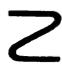
\includegraphics[keepaspectratio]{images/part001_c7194320.jpg}}

我们注意到，若 M 与 N 是 Hausdorff 拓扑向量空间 E 中任意两个闭向量子空间，则 \(M + N\) 在 E 中不一定是闭的，* 即使 E 是 Hilbert 空间 *（cf.~IV, 第 64 页, 习题 13, d)）。

命题 3. --- 设 E 是完备非离散赋值除环 K 上的一个拓扑向量空间。设 M 是 E 中具有有限余维数 n 的闭向量子空间。则 M 在 E 中的每个代数补子空间 N 也是拓扑补。

在 N 中，集合 \(\{0\}\) 是闭的，因为它是 N 与在 E 中为闭的集合 M 的交；于是 N 是 Hausdorff 的。由于 E/M 也是 Hausdorff 的，N 到 E/M 上的典范映射（它线性且双射）是双连续的（I, 第 14 页, cor. 2），由此命题得证。

推论. --- 设 E 与 F 是完备非离散赋值除环上的两个拓扑向量空间。若 F 是 Hausdorff 的且有限维，则 E 到 F 上的每个连续线性映射都是严格态射。

注记. --- 第 2, 3 目的结果当 K 是离散除环时不再成立。例如，设 \(K_{1}\) 是非离散赋值除环，K 是通过给 \(K_{1}\) 赋以 \(K_{1}\) 上的非真绝对值而得到的离散除环。于是 \(K_{1}\) 是 K 上的一个一维拓扑向量空间，但它不同构于 \(K_{s}\)。不过，我们可以证明：只要对所考虑的拓扑向量空间加上具有 0 的均衡邻域基本系这一性质（即满足 \(K.V = V\) 的邻域 V）（I, 第 27 页, 习题 14），第 2, 3 目的结果即使当 K 是离散的也成立；正如上例所示，这一条件（当 K 是非离散赋值除环时它总被满足，cf.~I, 第 7 页, prop. 4）并非对 K 上的所有拓扑向量空间都成立。

